\documentclass[9pt]{beamer}
\usepackage[utf8]{inputenc}
\usepackage[T1]{fontenc}
\usepackage[russian]{babel}
\usepackage{graphicx}
\usepackage{tikz}
\usepackage{pifont}
\usetheme{Dresden}
\usecolortheme{beaver}
\setbeamerfont{block title}{size=\normalsize}
\title[Electric motors data analysis]{\huge Electric motors data analysis}
\author[Snesarevskii, Belli, Biava, Dragi\'c, Kalenova] {{\Large Group 8:\\}Viktor Snesarevskii\\Edoardo Belli\\Guendalina Biava\\Ozrenka Dragi\'c\\Madina Kalenova}
\date{March-April 2018}

\begin{document}
	\begin{frame}
	\titlepage
	\vfill
	\begin{flushright}
		
\includegraphics[height=.7cm]{abb.png}
	\end{flushright}
\end{frame}
\begin{frame}{Dataset}
\begin{itemize} %[<+->]
\item Measurements of torque and current from electric motors
\item Time-series data with frequency 20KHz
\item Data taken from 5 distinct motors in AC and DC modes
\item Each data sample is one recorded operation
\item Operations are recorded while motor is working properly, then a fault is induced and the same operations are recorded again 
\item In total 1066 AC samples, 924 DC samples
\end{itemize}
\end{frame}
\begin{frame}{Data Example}
\begin{figure}\centering
\begin{tabular}{|c|c|}\hline
\textbf{Torque} & \textbf{Current} \\\hline
16.693&0.023\\\hline
16.739&0.019\\\hline
16.823&0.010\\\hline
16.810&0.007\\\hline
16.823&-0.002\\\hline
16.849&-0.010\\\hline
16.992&-0.018\\\hline
17.108&-0.033\\\hline
17.290&-0.035\\\hline
17.297&-0.052\\\hline
\end{tabular}\end{figure}
\end{frame}
\begin{frame}{Main Goals}
3 main goals:
\begin{itemize} %[<+->]
\item {\large Motor Classification}\\
Can we identify a motor by a recorded operation?
\item {\large Fault Classification}\\
Can we group faults?
\item {\large Fault Prediction}\\
Can we predict the state of motor by a recorded operation?
\end{itemize}
\end{frame}
\begin{frame}{First Steps}
\textbf{First problem} --- data is very high-dimensional ($p\approx 10^5$)\\
\textbf{Solution} --- do PCA first to select the most important moments\\[.4cm]
\textbf{Then} --- data exploration\\
For example, do faulty and working operations have the same or different mean, distribution etc
\end{frame}
\begin{frame}{Before PCA}
\textbf{\large Loading data into frame}\\
\textbf{Problem} --- different lengths of data samples\\
\textbf{Solution} --- cut all samples to minimal length value
\end{frame}
\begin{frame}{PCA}
PCA results go here
\end{frame}
\begin{frame}{Data Properties}
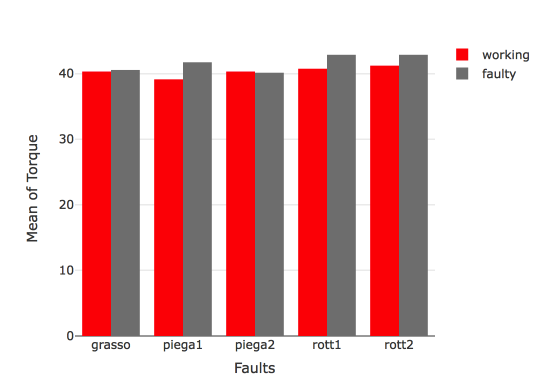
\includegraphics[width=6cm, height= 5.5cm]{TorqueMean.png}
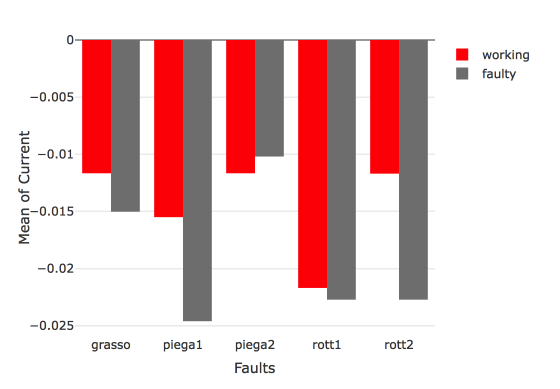
\includegraphics[width=6cm, height=5.5cm]{CurrentMean.png}
\end{frame}
\begin{frame}{Conclusions}
What we got so far
\end{frame}
\frame{\centering\huge Questions?}
\end{document}